% Adjust these for the path of the theme and its graphics, relative to this file
%\usepackage{beamerthemeFalmouthGamesAcademy}
\usepackage{../../beamerthemeFalmouthGamesAcademy}
\usepackage{multimedia}
\graphicspath{ {../../} }

% Default language for code listings
\lstset{language=C++,
        morekeywords={each,in,nullptr}
}

% For strikethrough effect
\usepackage[normalem]{ulem}
\usepackage{wasysym}

% https://tex.stackexchange.com/a/42620
\usepackage{pifont}% http://ctan.org/pkg/pifont
\newcommand{\cmark}{\ding{51}}%
\newcommand{\xmark}{\ding{55}}%


\usepackage{pdfpages}

% http://www.texample.net/tikz/examples/state-machine/
\usetikzlibrary{arrows,automata}

\newcommand{\modulecode}{COMP702}\newcommand{\moduletitle}{Classical Artificial Intelligence}\newcommand{\sessionnumber}{1}

\hypersetup{
pdftex,
pdftitle=\sessionnumber: What Is AI?,
pdfauthor=Ed Powley,
pdfdisplaydoctitle,
pdflang=en-GB
}

\begin{document}
\title{\sessionnumber: What Is AI?}
\subtitle{\modulecode: \moduletitle}

\frame{\titlepage} 

\part{What is ``Classical'' AI?}
\frame{\partpage}

\begin{frame}{What is AI?}
    \begin{itemize}
        \pause\item[\xmark] Simulating human brains or human intelligence
        \pause\item[\cmark] Performing tasks by machine (or by software) which would ordinarily require human intelligence
        \pause\item[\cmark] Making decisions to achieve goals
    \end{itemize}
\end{frame}

\begin{frame}{What is AI?}
    \begin{itemize}
        \pause\item[\xmark] Programming machines to learn by themselves
        \pause\item[\cmark] Machine learning is an important sub-field of AI, but there are many other AI techniques
    \end{itemize}
\end{frame}

\begin{frame}{What is AI?}
    \begin{itemize}
        \pause\item[\xmark] Programming machines to possess general intelligence, self-awareness, consciousness
        \pause\item[\cmark] Maybe one day, but for now this is pure sci-fi
        \pause\item[\cmark] Programming machines to carry out (or learn to carry out) a specific type of task
    \end{itemize}
\end{frame}

\begin{frame}{What is classical AI?}
    \begin{itemize}
        \pause\item A.k.a. \textbf{Good Old Fashioned AI}
        \pause\item A.k.a. \textbf{Symbolic AI}
        \pause\item Based on symbolic (``human-readable'') representations of problems, logical systems, search spaces
        \pause\item As opposed to machine learning, evolutionary algorithms etc which tend to be ``black boxes''
    \end{itemize}
\end{frame}

\begin{frame}{Applications of AI in games}
	\begin{itemize}
		\pause\item Enemies and other NPCs
		\pause\item Opponents in $\{$board, card, strategy$\}$ games
		\pause\item Automated playtesting
		\pause\item Directors, hints, adaptive difficulty
		\pause\item Procedural content generation
		\pause\item Content production tools
		\pause\item Procedural narrative
		\pause\item Agent-based simulations
		\pause\item ...
	\end{itemize}
\end{frame}

\begin{frame}{Why game AI?}
	\begin{itemize}
		\pause\item Games are a useful testbed for new AI technologies
		\pause\item Game theory is a useful mathematical abstraction for many types of problem
		\pause\item Game AI is more than pure problem solving --- game AI needs to create an entertaining experience
	\end{itemize}
\end{frame}

\part{AI architectures}
\frame{\partpage}

\begin{frame}{Rule-based AI}
	\begin{itemize}
		\pause\item Generally implemented as \texttt{if} statements or event-based triggers
		\pause\item Triggers can be complicated e.g.\ based on raycasts
	\end{itemize}
\end{frame}

\begin{frame}{Finite state machines}
	\begin{center}
		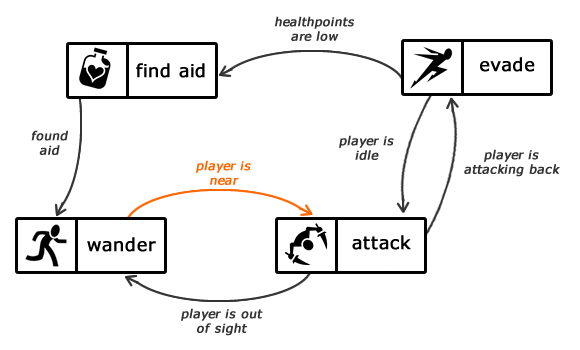
\includegraphics[width=\textwidth]{fsm_enemy_brain}
		% https://gamedevelopment.tutsplus.com/tutorials/finite-state-machines-theory-and-implementation--gamedev-11867
	\end{center}
\end{frame}

\begin{frame}{Behaviour trees}
	\begin{center}
		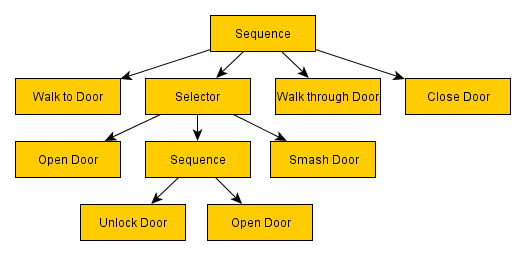
\includegraphics[width=\textwidth]{behaviour_tree}
		% https://www.gamasutra.com/blogs/ChrisSimpson/20140717/221339/Behavior_trees_for_AI_How_they_work.php
	\end{center}
\end{frame}

\begin{frame}{Multi-agent approaches (e.g.\ flocking)}
	\begin{center}
		
\includegraphics[width=\textwidth]{flocking}
		% https://www.youtube.com/watch?v=5p6OAEVKw-0
	\end{center}
\end{frame}

\begin{frame}{Game tree search}
	\begin{center}
		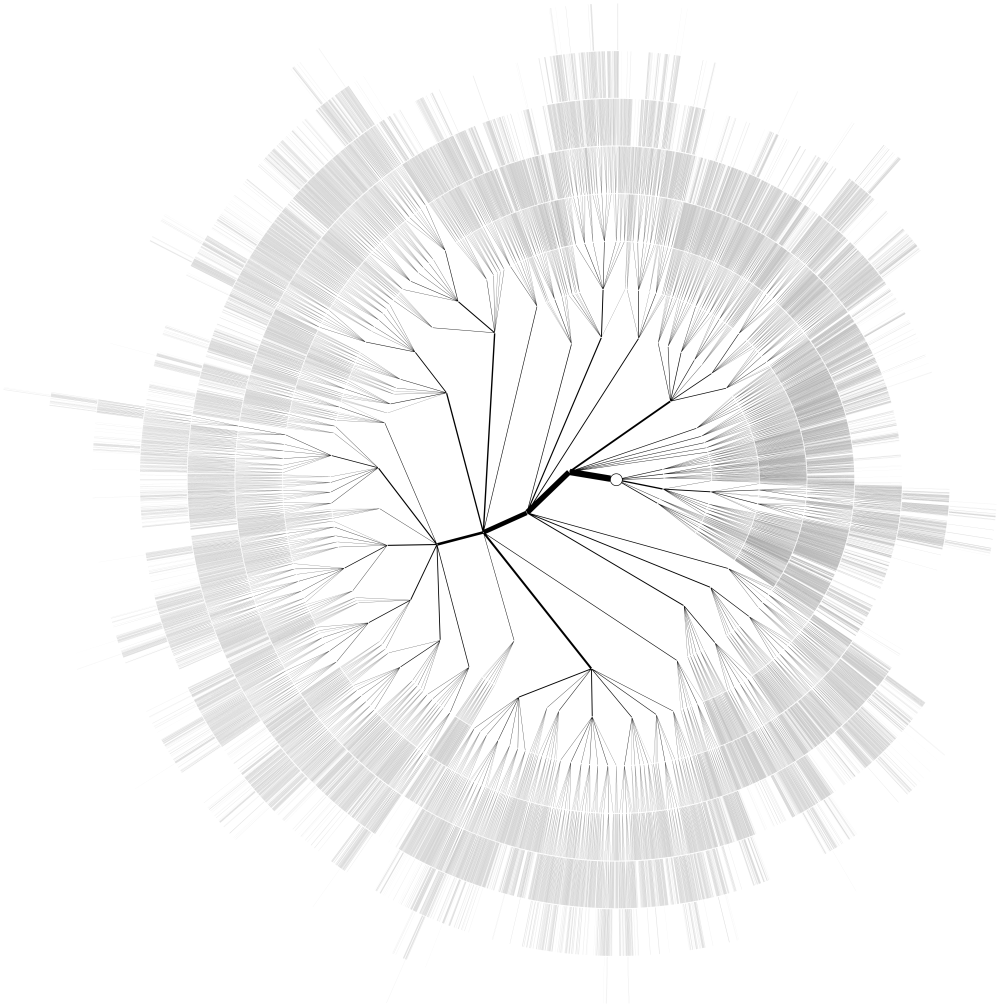
\includegraphics[height=0.7\textheight]{mcts}
	\end{center}
\end{frame}

\begin{frame}{Planning}
	\begin{center}
		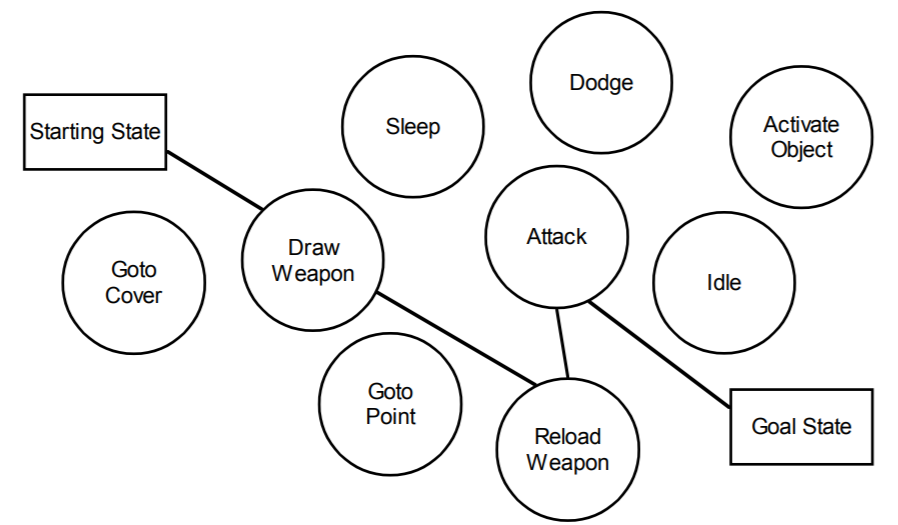
\includegraphics[width=\textwidth]{goap}
		% http://alumni.media.mit.edu/~jorkin/GOAP_draft_AIWisdom2_2003.pdf
	\end{center}
\end{frame}

\begin{frame}{Machine learning}
	\begin{center}
		\colorbox{white}{
			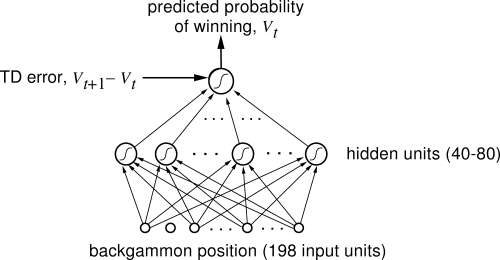
\includegraphics[width=0.7\textwidth]{tdgammon}
		}
		% https://users.auth.gr/kehagiat/Research/GameTheory/12CombBiblio/BackGammon.html
	\end{center}
\end{frame}

\begin{frame}{AI architectures}
	\begin{itemize}
		\pause\item Can roughly be divided into \textbf{hand-authored}...
			\begin{itemize}
				\pause\item Rule-based, FSM, behaviour trees
			\end{itemize}
		\pause\item ... and \textbf{computational intelligence}
			\begin{itemize}
				\pause\item Search, planning, machine learning
			\end{itemize}
		\pause\item Do you want to \textbf{design} the AI behaviours yourself,
			or do you want them to \textbf{emerge} from the system?
		\pause\item Predictability and authorial control versus adaptability and novelty
		\pause\item Can also combine the two, e.g.\ use a rule-based system to constrain a CI system
	\end{itemize}
\end{frame}

%\part{Agents}
\frame{\partpage}

\begin{frame}{Agents}
    \begin{center}
        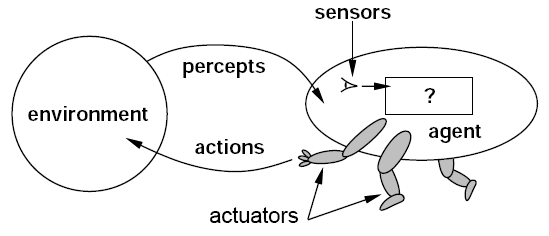
\includegraphics[width=0.7\textwidth]{agent}

        \vspace{2ex}

        \pause An \textbf{agent} is anything which perceives an \textbf{environment} through \textbf{sensors},
            and acts upon that environment through \textbf{actuators}.
    \end{center}
\end{frame}

\begin{frame}{Performance}
    \begin{itemize}
        \pause\item An ``intelligent'' agent moves towards some kind of \textbf{goal}
        \pause\item The goal is an \textbf{environment state} (or a set of states)
        \pause\item A \textbf{performance measure} evaluates a given state for how well it fits the goal
    \end{itemize}
\end{frame}

\begin{frame}{PEAS}
    For each example of an agent, what are the \underline{P}erformance measure,
        \underline{E}nvironment, \underline{A}ctuators and \underline{S}ensors?
    
    % \begin{itemize}
    %     \pause\item A Roomba
    %     \pause\item A self-driving car
    %     \pause\item A chatbot
    %     \pause\item A factory robot
    %     \pause\item An enemy in an FPS game
    %     \pause\item A chess AI
    %     \pause\item A human
    % \end{itemize}
\end{frame}

\begin{frame}{Types of environment}
    \begin{itemize}
        \pause\item Environments come with many different properties
        \pause\item These properties influence the choice of AI architecture we use to build agents
    \end{itemize}
\end{frame}

\begin{frame}{Observability}
    \begin{itemize}
        \pause\item \textbf{Fully observable}: the agent's sensors give it full information about the state of the environment
        \pause\item \textbf{Partially observable}: some aspects of the environment state are not visible to the agent's sensors
        \pause\item E.g.\ a chess game is fully observable, a poker game is partially observable
    \end{itemize}
\end{frame}

\begin{frame}{Number of agents}
    \begin{itemize}
        \pause\item \textbf{Single agent}: our agent is the only one in the environment
        \pause\item \textbf{Multi-agent}: there is more than one agent
        \pause\item \textbf{Cooperative}: all agents share the same performance measure
        \pause\item \textbf{Competitive}: agents' performance measures are in opposition to each other
            (i.e.\ if one agent ``wins'', another ``loses'')
    \end{itemize}
\end{frame}

\begin{frame}{Determinism}
    \begin{itemize}
        \pause\item \textbf{Deterministic}: the next state of the environment is completely determined by the current state and by the agent's action
        \pause\item \textbf{Stochastic}: there is some aspect of randomness in determining the next state
        \pause\item E.g.\ chess is deterministic; any board game involving dice rolls or random card draws is stochastic
    \end{itemize}
\end{frame}

\begin{frame}{Dynamicity}
    \begin{itemize}
        \pause\item \textbf{Static}: the environment does not change while the agent is deliberating
        \pause\item \textbf{Dynamic}: the environment changes constantly
        \pause\item E.g.\ most board games are static, most (non turn-based) video games are dynamic
    \end{itemize}
\end{frame}

\begin{frame}{Discreteness}
    \begin{itemize}
        \pause\item \textbf{Discrete}: time, percepts and actions are all discrete
            (from a finite set of possibilities or ``integer valued'')
        \pause\item \textbf{Continuous}: at least one of these is not discrete
            (``float valued'')
        \pause\item Continuous problems are hard so we sometimes \textbf{discretise} them
    \end{itemize}
\end{frame}

\begin{frame}{Known or unknown}
    \begin{itemize}
        \pause\item Are all the details of the environment \textbf{known} to the AI designer?
        \pause\item For a game or simulation: probably \textbf{yes}
            (unless someone else made it and we don't have the source code)
        \pause\item For the real world: technically \textbf{no}
            (but we have physics, sociology, economics etc to give us good approximations)
    \end{itemize}
\end{frame}

\begin{frame}{Agents and AI}
    \begin{itemize}
        \pause\item The ideas of agents and environments are a useful frame for designing AI
        \pause\item All(?) AI problems can be expressed in terms of creating an agent
            that optimises some performance measure in some environment
        \pause\item Agent design boils down to: given a \textbf{percept} (and possibly some \textbf{memory} of past percepts/actions),
            choose the best \textbf{action} to take now
    \end{itemize}
\end{frame}


\end{document}
